\documentclass{article}
\usepackage{tkz-euclide}
\usepackage{tikz}
\usepackage{textpos}
\usepackage{tikz}
\usepackage{tikz-3dplot}
\usepackage{tkz-euclide}
\usepackage{chemfig}

\begin{document}

\begin{scriptsize}
		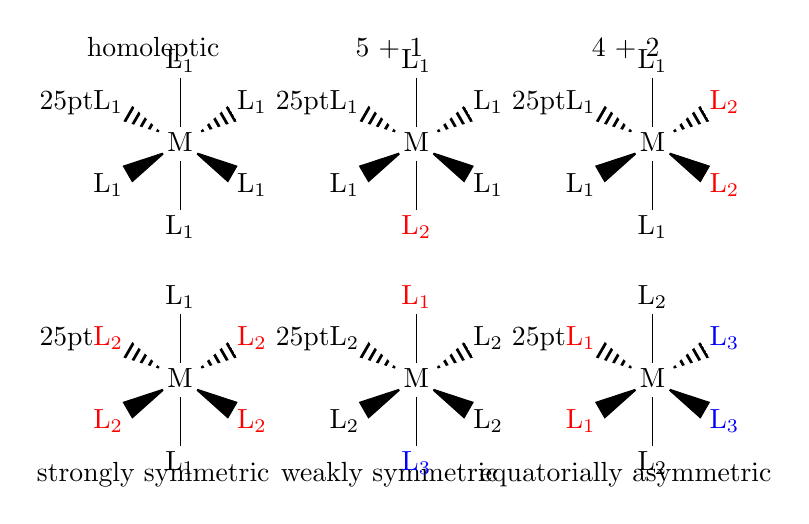
\begin{tikzpicture}
%		\draw[thick, use as bounding box](-1,-1) rectangle (10,5);
		% % % %
		
		\node [color=black] (lab11) at (1,4.7) {homoleptic};
		
		\node (met) at (1,3.5){\setatomsep{25pt}\chemfig{{L_1}>:[:-30]{{\color{black}M}}([:-150]<{L_1})([:90]-{{L_1}})(<:[:30]L_1)(<[:-30]L_1)([:-90]
				-{{L_1}})}};
		
		% % %
		\node [color=black] (lab21) at (4,4.7) {5 + 1};
		\node (met21) at (4,3.5){\setatomsep{25pt}\chemfig{{L_1}>:[:-30]{{\color{black}M}}([:-150]<{L_1})([:90]-{{L_1}})(<:[:30]L_1)(<[:-30]L_1)([:-90]-{\color{red}{L_2}\color{black}})}};
		
		
		% % %
		\node [color=black] (lab12) at (1,-0.7) {strongly symmetric};
		
		\node (met12) at (1,0.5){\setatomsep{25pt}\chemfig{\color{red}{L_2}\color{black}>:[:-30]{{\color{black}M}}([:-150]<\color{red}{L_2})([:90]-{ \color{black}{L_1}})(<:[:30]\color{red}{L_2\color{black}})(<[:-30]{\color{red}L_2}\color{black})([:-90]-{{L_1}})}};
		
		
		% % %
		\node [color=black] (lab12) at (4,-0.7) {weakly symmetric};
		
		\node (met) at (4,0.5){\setatomsep{25pt}\chemfig{{L_2}>:[:-30]{{\color{black}M}}([:-150]<{L_2})([:90]-{\color{red}{L_1}})(<:[:30]L_2)(<[:-30]L_2)([:-90]-{\color{blue}{L_3}})}};
		
		
		% % %
		\node [color=black] (lab12) at (7,4.7) {4 + 2};
		\node (met) at (7,3.5){\setatomsep{25pt}\chemfig{{L_1}>:[:-30]{{\color{black}M}}([:-150]<{L_1})([:90]-{{L_1}})(<:[:30]\color{red}{L_2})(<[:-30]\color{red}{L_2})([:-90]-{{L_1}})}};
		
		
		% % %
		\node [color=black] (lab12) at (7,-0.7) {equatorially asymmetric};
		
		\node (met) at (7,0.5){\setatomsep{25pt}\chemfig{{\color{red}{L_1}}>:[:-30]{{\color{black}M}}([:-150]<{\color{red}{L_1}})([:90]-{\color{black}{L_2}})(<:[:30]\color{blue}{L_3})(<[:-30]\color{blue}{L_3})([:-90]-{{L_2}})}};
		\end{tikzpicture}
	\end{scriptsize}

\end{document}